\chapter[Elements]{Elements} 
\label{chp2_elements} 

This chapter presents examples of how to cite some references, how to use figures, tables, equations, algorithms and other explanatory elements.

%-----------------------------------
\section{Citations}

The Standard \texttt{ABNT NBR 10520: 2002} describes that \index{quotations} short direct quotations with (less than three lines) must be described with ``double quotes'' around it. Otherwise, \index{direct quotations}long direct quotations (up to three lines) must be highlighted with a 4cm indentation of the left margin, with lower than the used text and without the quotation marks. To do this, use the citation environment, as the example:

\begin{citacao}
For example, if the probability of an event is not known with precision, then it may be characterized linguistically as, say, quite likely, not very unlikely, highly unlikely, etc., where quite likely, not very unlikely and highly unlikely are interpreted as labels of fuzzy subsets of the unit interval. Such subsets may be likened to ball-parks without sharply defined boundaries which serve to provide an approximate rather than exact characterization of the value of a variable \citep{zadeh1976fuzzy}.
\end{citacao}

%-----------------------------------
\section{References}

Throughout your dissertation or thesis, you can use the references in two main ways: 1) automatically link from bibliographic management softwares Mendeley\footnote{www.mendeley.com}, Zotero\footnote{www.zotero.org}, CiteULike\footnote{www.citeulike.org/} and 2) add \index{references} references in your own .bib file, as \texttt{references.bib} used in this document. To facilitate your work, it is suggested to get the link in Google Scholar (but you need to check them, because not all the references are correct).
\index{enumerate items}

Some examples of \index{citations} citations as well as example of enumerations:

\begin{enumerate}%[label=(\roman*)]
\itemsep0em %Reduce space between enumerated items
    \item Multicriteria decision making methods have been largely used in the literature. A comparative study between Vikor and Topsis methods were proposed by \cite{opricovic2004comparative};
    
    \begin{enumerate}
    \itemsep0em 
        \item One;
        \item Two;
        
        \begin{enumerate}
        \itemsep0em 
            \item Cachaça;
            \item Caipirinha.
        \end{enumerate}
        
        \item Three.
    \end{enumerate}
    
    \item According to \cite{Babington1993book,Harwood1993mastersthesis} and \cite{Joslin1993thesis}, the multicriteria decision making methods have been largely used in the literature. 
    \item According to \cite{Babington1993book} and \cite{opricovic2004comparative}, the multicriteria decision making methods have been largely used in the literature. %Tip: when you are going to use two or more citations, keep them in order of publication year.
    \item Multicriteria decision making methods have been largely used in the literature \citep{Isley1990misc,Babington1993book,Adams1993journal,opricovic2004comparative}.
    \item Support Vector Machine (SVM) has achieved an average accuracy of 94.67\% in the recognition of Brazilian Sign Language signals \citep{rezende2017analise}.
\end{enumerate}

In the file \url{http://linorg.usp.br/CTAN/macros/latex/contrib/abntex2/doc/abntex2cite.pdf} you can find more examples.


%-----------------------------------
\section{Equations}
\index{equations}

Simple equations can be described inside the sentences or separately. See the two examples.

The mass-energy equivalence is described by the famous equation $E=mc^2$ discovered in 1905 by Albert Einstein. 
In natural units ($c = 1$), the formula expresses the identity represented as follows in \eqref{eq_massenergy}
 
\begin{equation}
\label{eq_massenergy}
E=m
\end{equation}

In your text, when you need to cite this equation, rather than you use \texttt{ref}, use \texttt{eqref}. For example: $\hdots$ represented in \eqref{eq_exemplo} blah blah blah. It can be seen that the latter does not a label for it, then it cannot be invoked lately, already the former can.

\begin{equation}
\label{eq_exemplo}
f'(x) = \int^{x^2}_{x^{-1}} xdx 
\end{equation}

In addition, you can use an infinity of things, since the \LaTeX is an excellent tool to deal with equations.


%-----------------------------------
\section{Figures}
\index{figures}

The Figure \ref{fig_gatofofo} is just an example of a cute cat copied from somewhere on the internet. You can use PNG, JPG ou PDF format. It is important to note that figure captions are below their contents. Taking into consideration the practicality (and time), it is indicated to use suggestive names to the figures, equations and others labels that you are going to use. This will greatly facilitate your life while writing your dissertation or thesis.

\begin{figure}[htb] 
    \centering
    
\includegraphics[width=0.5\textwidth]{figures/gatofofo.PNG}
    \caption{Cute cat.}
    \label{fig_gatofofo}
    \caption*{Source: \cite{Babington1993book}}
\end{figure}


You also use subfigures to take your document more organized. The Figure \ref{fig_subfigname} illustrates an example. To cite one specific \index{subfigure} sub-figure you can do this either this \ref{subfig_cutecat} or \ref{subfig_cutestdog}.

\begin{figure}[!ht]
    \centering
    \caption{Caption superior.}
        \subfloat[Cute cat]{
            
\includegraphics[width=0.3\textwidth]{figures/gatofofo.PNG}
            \label{subfig_cutecat}
        }\qquad
        \subfloat[Custest dog]{
            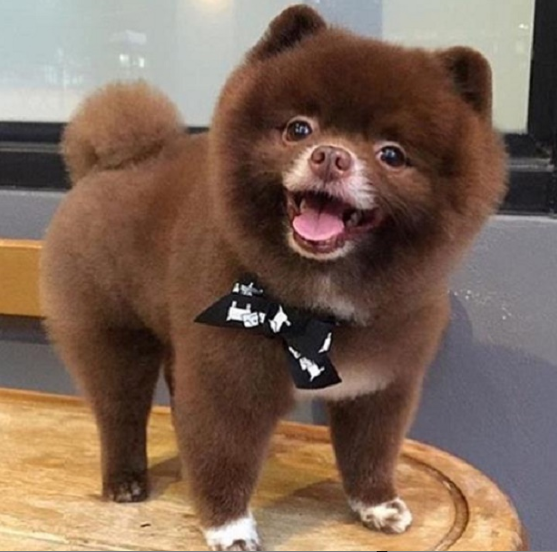
\includegraphics[width=0.3\textwidth]{figures/cachorrofofo.PNG}
            \label{subfig_cutestdog}
        }
    \label{fig_subfigname}
\end{figure}


See \texttt{CTAN: Package subfigure}\footnote{https://ctan.org/pkg/subfigure} for more information. It is possible, yet, to include figures using the package \texttt{subfig}, see e.g. \url{https://tex.stackexchange.com/questions/37581/latex-figures-side-by-side}.

%-----------------------------------
\section{Inserting Outputs Commands and Codes}
\index{output commands}

Excerpts from configuration files and application code may be inserted as figure, as shown in \ref{fig_exemplocomando}. 

To commands and configuration files, it is recommended to use the package \texttt{fancyvrb}. Now, to insert code, you should use the package \texttt{listings} which presents a better presentation of its. In addiction, these both packages allow you insert text/code in external files, without incluse directly in the \LaTeX file.

\begin{figure}[!htb]
\centering
\caption{Inserting Command} 
\begin{Verbatim}[fontsize=\small]
$ dir thesis*
-rw-r--r--  1 joukim users   3650 Set 12 17:56 dissertation.aux
-rw-r--r--  1 joukim users   6366 Set 12 17:43 dissertation.bbl
-rw-r--r--  1 joukim users    290 Set 12 17:56 dissertation.lof
-rw-r--r--  1 joukim users  27937 Set 12 17:56 dissertation.log
-rw-r--r--  1 joukim users    194 Set 12 17:56 dissertation.lot
-rw-r--r--  1 joukim users    715 Set 12 17:56 dissertation.out
-rw-r--r--  1 joukim users 159243 Set 12 17:56 dissertation.pdf
-rw-r--r--  1 joukim users   4559 Set 12 17:47 dissertation.tex
-rw-r--r--  1 joukim users    964 Set 12 17:56 dissertation.toc
\end{Verbatim} 
%$ - esse comentário é para não confundir editor de texto
{\small Source: Blah blah blah, 2018} 
\label{fig_exemplocomando} 
\end{figure}

%-----------------------------------
\section{Tables}
\label{sec_tabelas}

The subsections \ref{subsec_tabsimples} and \ref{subsec_longtable} present examples of \index{table} short table (Table \ref{tab_shorttable}) and long table (Table \ref{tab_longtable}).

%-----------------------------------
\subsection{Example of a Short Table}
\label{subsec_tabsimples}
\index{short table}

We follow the simple rule: horizontal lines only to emphasize the title and in the last line and without vertical lines, as illustrated in Table \ref{tab_shorttable} and Table \ref{tab_longtable} (in Appendix, \ref{appendix}).

To create the tables, we strongly suggest the use of website \texttt{tablegenerator}, available in \url{https://www.tablesgenerator.com/}. It will save your life.

More tips: text should be aligned to the left and keep the numbers with the same number of decimal places and aligned to the right.

\begin{table}[htb]
    \centering
    \caption{Example of a Short Table}
    \label{tab_shorttable}
    \begin{tabular}{lrrr}
    \hline
        Description          & \multicolumn{1}{c}{Value 1} & \multicolumn{1}{c}{Value 2} & \multicolumn{1}{c}{Value 3} \\ \hline
        Cachaça              & 1352,70                     & 1,22                        & 1358,00                     \\
        Caipirinha           & 2005,00                     & 75,21                       & 6873,11                     \\
        Jeropinga            & 8648,00                     & 5,45                        & 852,00                      \\
        Bluepinga            & 4587,55                     & 153,00                      & 53468,00                    \\
        Pagar com Mastercard & 0,00                        & 0,00                        & 0,00                        \\ \hline
    \end{tabular}
\end{table}

%-----------------------------------
\subsection{Example of a Long Table}
\label{subsec_longtable}
\index{long table}

This  long table is in landscape view for better visualization of the information contained. For organization reasons it was sent to the appendix, Section \ref{apendiceA}.


%-----------------------------------
\section{Algorithms}

This section gives an example of Euclid’s \index{algorithm} algorithm shown in \ref{alg_euclid}.

\begin{algorithm}
\caption{My algorithm}\label{alg_euclid}
    \begin{algorithmic}[1]
    \Procedure{MyProcedure}{}
    \State $\textit{stringlen} \gets \text{length of }\textit{string}$
    \State $i \gets \textit{patlen}$
    \BState \emph{top}:
    \If {$i > \textit{stringlen}$} \Return false
    \EndIf
    \State $j \gets \textit{patlen}$
    \BState \emph{loop}:
    \If {$\textit{string}(i) = \textit{path}(j)$}
    \State $j \gets j-1$.
    \State $i \gets i-1$.
    \State \textbf{goto} \emph{loop}.
    \State \textbf{close};
    \EndIf
    \State $i \gets i+\max(\textit{delta}_1(\textit{string}(i)),\textit{delta}_2(j))$.
    \State \textbf{goto} \emph{top}.
    \EndProcedure
    \end{algorithmic}
\end{algorithm}

%-----------------------------------
\section{Some additional links}

In addition, additional links are given bellow:

\begin{itemize}
    \item The \texttt{tocbibind}
package\footnote{http://linorg.usp.br/CTAN/macros/latex/contrib/tocbibind/tocbibind.pdf} - in English.
    \item The \texttt{tocloft}
package\footnote{http://linorg.usp.br/CTAN/macros/latex/contrib/tocloft/tocloft.pdf} - in English.
    \item The \texttt{abntex2cite} package\footnote{http://linorg.usp.br/CTAN/macros/latex/contrib/abntex2/doc/abntex2cite.pdf} - in Portuguese.

\end{itemize}